\documentclass{article}


\usepackage{arxiv}

\usepackage{graphicx}
\usepackage{amsmath}
\usepackage{amssymb}
\usepackage{epstopdf}
\usepackage{comment}

\newcommand{\beqn}{\begin{equation}}
\newcommand{\eeqn}{\end{equation}}
\newcommand{\req}[1]{Eq.\,(\ref{#1})}
\newcommand{\TeV}{\text{ TeV}}
\newcommand{\GeV}{\text{ GeV}}
\newcommand{\MeV}{\text{ MeV}}
\newcommand{\keV}{\text{ keV}}
\newcommand{\eV}{\text{ eV}}
\newcommand{\meV}{\text{ meV}}


%\topmargin=-0.5cm
%\pagestyle{plain}  % COMMENT OUT 
%\thispagestyle{plain}
%\footskip=0.8cm



\title{\boldmath Composition of the Universe}

\author{Johann Rafelski and Jeremiah Birrell}


\begin{document}

\maketitle

 



\section{Composition of the Universe}\label{sec:E_dens}
The composition of the Universe, in terms of energy density fractions of various particle species, gives valuable insight into the history of the Universe.  In Figure \ref{fig:energy_frac} we begin on the right at the end  of the QGP era.  The first dotted vertical line shows the QGP phase transition and hadronization, near $T=150\MeV$. The hadron era proceeds with the disappearance of muons, pions, and heavier hadrons.  This constitutes a reheating period, with energy and entropy from these particles being transferred to the remaining $e^\pm$, photon, neutrino plasma.   The black circle near $T=115\MeV$ denotes our change from $2+1$-flavor lattice QCD data for the hadron energy density, taken from Borsanyi et al.~\cite{Borsanyi:2013bia}, to an ideal gas model at lower temperature.  We note that the hadron ideal gas energy density matches the lattice results to less than a percent at $115\MeV$. 

%%%%%%%%%%%%%%%%%%%%%%%%%%%%%%%%%%%%%%%
\begin{figure} 
\centerline{\hspace*{0.4cm}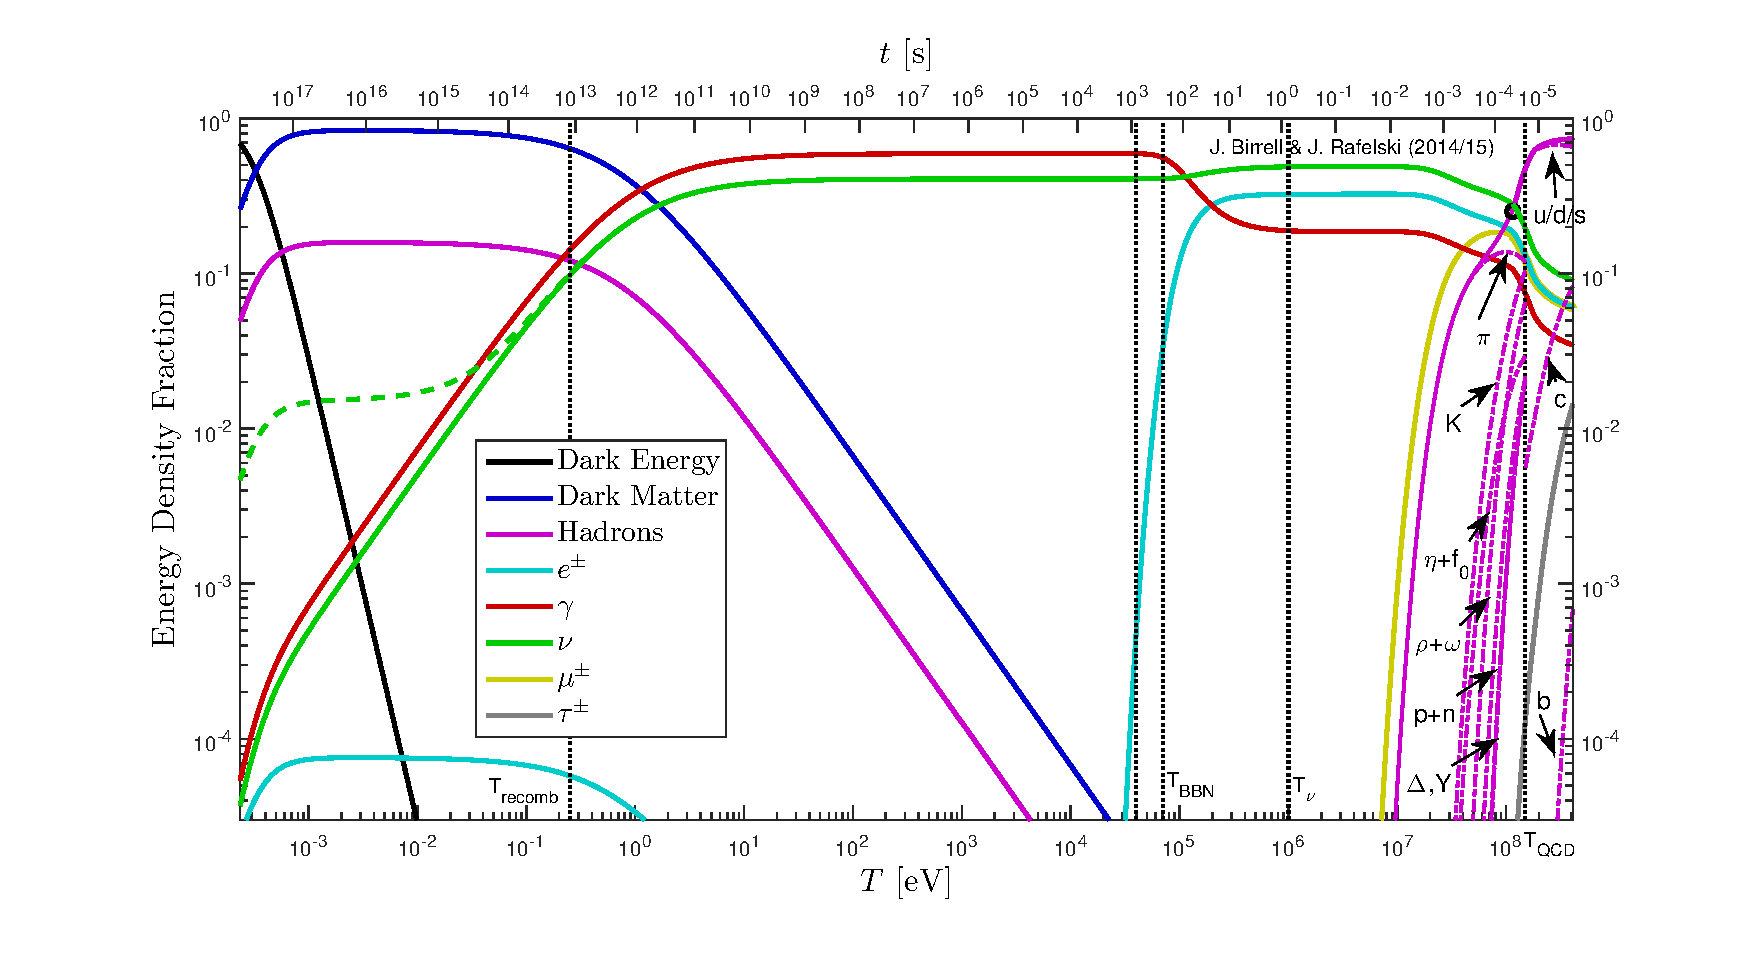
\includegraphics[height=11cm]{./plots/energy_fractions.eps}}
\centerline{\hspace*{0.4cm}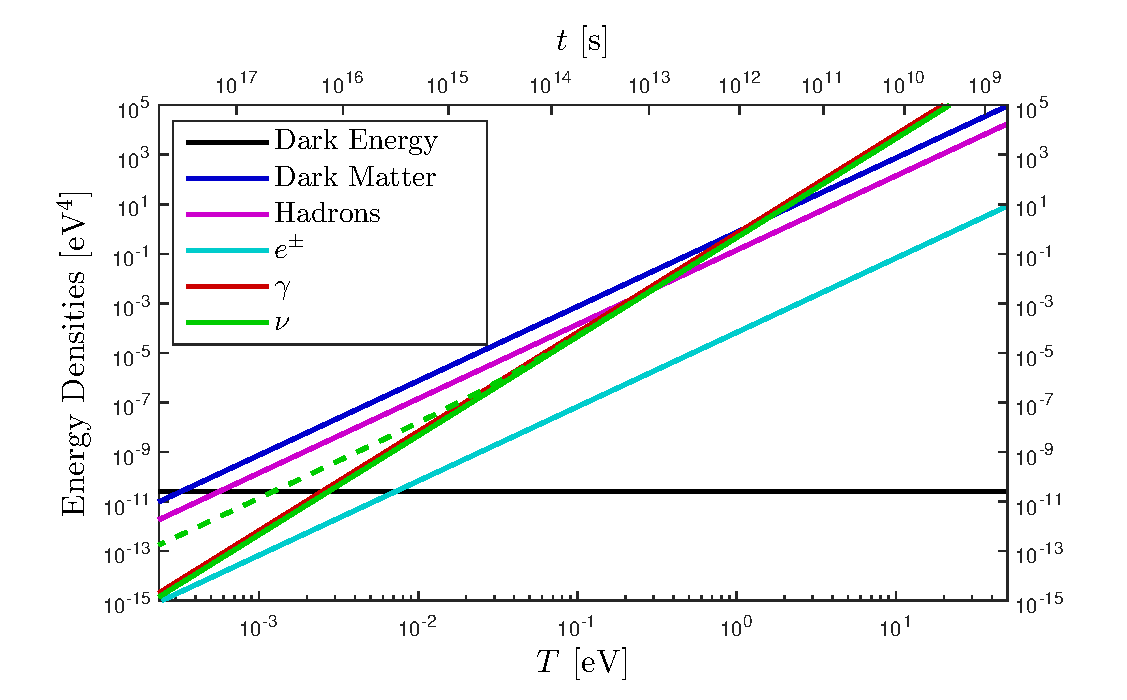
\includegraphics[height=8.5cm]{./plots/energy_densities.eps}}
\caption{Current era: $69\%$ dark energy, $26\%$ dark matter, $5\%$ baryons, $<1\%$ photons and neutrinos.  Solid neutrino line shows massless neutrinos while the dashed line shows $1$ massless and $2\times 0.1$ eV neutrinos (Neutrino mass choice is just for illustration.  Other values are possible).\label{fig:energy_frac}}
 \end{figure}
%%%%%%%%%%%%%%%%%%%%%%%%%%%%%%%%%%%%%%%



To the right of the QGP transition region, the solid hadron line shows the total energy density of quarks and gluons. From top to bottom, the dot-dashed hadron lines to the right of the transition show the energy density fractions of $2+1$-flavor (u,d,s) lattice QCD matter (almost indistinguishable from the total energy density), charm, and bottom (both in the ideal gas approximation).  To the left of the transition the dot-dashed lines show the  pion, kaon, $\eta+f_0$, $\rho+\omega$, nucleon,  $\Delta$, and Y  contributions to the energy fraction.


Continuing to the second vertical line at $T=O(1)$ MeV, we come to the annihilation  of $e^\pm$ and the photon reheating period.  Notice that only the photon energy density fraction increases here, as we assume here that neutrinos are already decoupled at this time and hence do not share in the reheating process, leading to a difference in photon and neutrino temperatures. This is not strictly correct but it is a reasonable simplifying assumption for the current purpose; see \cite{Mangano:2005cc,Birrell_orthopoly}.  We next pass through a long period, from $T=O(1)$ MeV until $T=O(1)$ eV, where the energy density is dominated by photons and free-streaming neutrinos.  BBN occurs in the approximate range $T=40-70\keV$ and is indicated by the next two vertical lines.  It is interesting to note that, while the hadron fraction is insignificant at this time, there is still a substantial background of $e^\pm$ pairs during BBN.  

 We then come to the beginning of the matter dominated regime, where the energy density is dominated by the combination of dark matter and baryonic matter.  This transition is the result of the redshifting of the photon and neutrino energy, $\rho\propto T^4$, whereas for non-relativistic matter $\rho\propto a^{-3}\propto T^3$.  Recombination and photon decoupling occurs near the transition to the matter dominated regime, denoted by the vertical line at $T=0.25\eV$.

Finally, as we move towards the present day CMB temperature of $T_{\gamma,0}=0.235$ meV on the left hand side, we have entered the dark energy dominated regime.  For the present day values, we have used the energy densities proscribed by the Planck parameters \req{Planck_params} and zero Universe spatial curvature.  The photon energy density is fixed by the CMB temperature $T_{\gamma,0}$ and the neutrino energy density is fixed by $T_{\gamma,0}$ along with the photon to neutrino temperature ratio and neutrino masses.  Both constitute $<1\%$ of the current energy budget.

The Universe evolution and total energy densities were computed using massless neutrinos, but  for comparison we show the energy density of massive neutrinos in the dashed green line. For the dashed line we used two neutrino flavors with masses $m_\nu=0.1\eV$ and one massless flavor.  Note that the inclusion of neutrino mass causes the leveling out of the neutrino energy density fraction during the matter dominated period, as compared to the continued redshifting of the photon energy.



\appendix

%%%%%%%%%%%%%%%%%%%%%%%%%%%%%%%%%%%%%%%%%%%%%%%%%%%%%%%%%%%%%%%
\section{Standard Cosmology}\label{cosmo}
%%%%%%%%%%%%%%%%%%%%%%%%%%%%%%%
Here we provide background on the standard  cosmological (FLRW-Universe) model that is used in the computation of the compositive of the universe over time. We use the spacetime metric
\beqn\label{metric}
ds^2=c^2dt^2-a^2(t)\left[ \frac{dr^2}{1-kr^2}+r^2(d\theta^2+\sin^2(\theta)d\phi^2)\right]
%g_{00}=1, \quad g_{rr}=-\frac{a^2}{1-kr^2}, \quad g_{\theta\theta}=-a^2r^2, \quad g_{\phi\phi}=-a^2 r^2\sin^2\theta
\eeqn
characterized  by the scale parameter $a(t)$  of a spatially homogeneous  Universe. The geometric parameter $k$ identifies the geometry of the spacial hypersurfaces defined by comoving observers. Space is a flat-sheet for the observationally preferred value $k=0$ \cite{Planck}. In this case it can be more convenient to write the metric in rectangular coordinates
\beqn\label{metric2}
ds^2=c^2dt^2-a^2(t)\left[ dx^2+dy^2+dz^2\right].
\eeqn
We will work in units where $\hbar=1,c=1$.

The global Universe dynamics can be characterized by two  quantities: the Hubble parameter  $H$, a strongly time dependent quantity on cosmological time scales,  and the deceleration parameter $q$:
\beqn\label{dynamic}
\frac{\dot a }{a}\equiv H(t) ,\quad \frac{\ddot a}{a}=-qH^2,\quad 
q\equiv -\frac{a\ddot a}{\dot a^2},\quad \dot H=-H^2(1+q). 
\eeqn

The Einstein equations are:
\beqn\label{Einstine}
G^{\mu\nu}=R^{\mu\nu}-\left(\frac R 2 +\Lambda\right) g^{\mu\nu}=8\pi G_N T^{\mu\nu},  
\quad R= g_{\mu\nu}R^{\mu\nu}.
\eeqn
Symmetry considerations imply that the stress energy tensor is determined by an energy density and an isotropic pressure
\begin{align}
 T^\mu_\nu =\mathrm{diag}(\rho, -P, -P, -P).
\end{align}
It is common to absorb the Einstein cosmological constant $\Lambda$ into the energy and pressure
\beqn\label{EpsLam}
\rho_\Lambda=\frac{\Lambda}{8\pi G_N}, \qquad P_\Lambda=-\frac{\Lambda}{8\pi G_N}
\eeqn
and we implicitly consider this done from now on.

Two dynamically independent equations arise using the metric \req{metric} in \req{Einstine}:
\beqn\label{hubble}
\frac{8\pi G_N}{3} \rho =  \frac{\dot a^2+k}{a^2}
=H^2\left( 1+\frac { k }{\dot a^2}\right),
\qquad
\frac{4\pi G_N}{3} (\rho+3P)  =-\frac{\ddot a}{a}=qH^2.
\eeqn
We can eliminate the strength of the interaction, $G_N$,  solving both these equations for ${8\pi G_N}/{3}$, and equating the result to find a relatively simple constraint for the deceleration parameter:
\beqn\label{qparam}
q=\frac 1 2 \left(1+3\frac{P}{\rho}\right)\left(1+\frac{k}{\dot a^2}\right).
\eeqn
For a spatially flat Universe, $k=0$, note that in a  matter-dominated era where $P/\rho<<1$ we have $q\simeq 1/2$; for a radiative Universe where $3P=\rho$ we find $q= 1 $; and  in a dark energy Universe in which $P=-\rho$  we find $q=-1$.  Spatial flatness is equivalent to the assertion that the energy density of the Universe equals the critical density
\begin{equation}\label{crit_density}
\rho=\rho_{\text{crit}}\equiv \frac{3H^2}{8\pi G_N}.
\end{equation}

 The CMB power spectrum is sensitive to the  deceleration parameter  and the presence of spatial curvature modifies $q$. The Planck results~\cite{Planck} constrain  the effective curvature energy density fraction,
\begin{equation}
\Omega_K\equiv1-\rho/\rho_{\text{crit}},
\end{equation}
to
\begin{equation}
|\Omega_K|<0.005.
\end{equation}
This indicates a nearly flat Universe. We will work here within an exactly spatially flat cosmological model, $k=0$.  


As must be the case for any solution of Einstein's equations,   \req{hubble} implies that the energy momentum tensor of matter is divergence free:
\beqn\label{divTmn}
T^{\mu\nu};_\nu =0 \Rightarrow -\frac{\dot\rho}{\rho+P}=3\frac{\dot a}{a}=3H.
\eeqn
A dynamical evolution equation for $\rho(t)$ arises once we combine \req{divTmn} with \req{hubble},  eliminating $H$.   Given an equation of state $P(\rho)$, solutions of this equation describes the dynamical evolution of matter in the Universe. In practice, we evolve the system in both directions in time.  On one side, we start in the present era with the energy density fractions fit by Planck data, 
\cite{Planck}
\begin{equation}\label{Planck_params}
H_0=67.74\text{km/s/Mpc},\hspace{2mm} \Omega_b=0.05,\hspace{2mm} \Omega_c=0.26, \hspace{2mm}\Omega_\Lambda=0.69,
\end{equation}
 and integrate backward in time.  On the other hand, we start in the QGP era with an equation of state determined by an ideal gas of SM particles, combined with a perturbative QCD equation of state for quarks and gluons \cite{Borsanyi:2013bia}, and integrate forward in time.

\section{Matter Content}\label{sec:matter}
In this work, matter will be modeled by a particle distribution function $f(t,x,p)$ that, roughly speaking, gives the probability of finding a particle per unit spacial volume per unit momentum space volume at a given time.  The distribution function gives the stress energy tensor, particle four-current, and entropy four-current via 
\begin{align}
T^{\mu\nu}(t,x)=&\frac{d}{(2\pi)^3}\int p^\mu p^\nu f(t,x,p) \sqrt{|g|}\frac{d^3p}{p_0},\\
n^\nu(t,x)=&\frac{d}{(2\pi)^3}\int p^\nu f(t,x,p) \sqrt{|g|}\frac{d^3p}{p_0},\\
s^\nu(t,x)=&-\frac{d}{(2\pi)^3}\int(f\ln(f)\pm(1\mp f)\ln(1\mp f))p^\nu\sqrt{|g|}\frac{d^3p}{p_0}
\end{align}
where the upper signs are for fermions, the lower for bosons, $d$ is the degeneracy of the particle, and $g$ is the determinant of the metric.  In a flat FRW Universe, the expressions for the  energy density, pressure, number density, and entropy density of a particle of mass $m$ are
\begin{align}\label{moments}
\rho=&\frac{d}{(2\pi)^3}\int f(t,x,p)Ed^3p,\hspace{2mm} E=\sqrt{m^2+p^2},\\
P=&\frac{d}{(2\pi)^3}\int f(t,x,p)\frac{p^2}{3E}d^3p,\\
n=&\frac{d}{(2\pi)^3}\int f(t,x,p) d^3p, \\
s=&-\frac{d}{(2\pi)^3}\int (f\ln(f)\pm(1\mp f)\ln(1\mp f)) d^3p.
\end{align}



\subsection{Equilibrium and Free-Streaming Distribution}\label{sec:free_stream}
Free-streaming is a type of non-equilibrium distribution that is significant in cosmology.  Here we outline its properties, including what distinguishes it from the equilibrium distributions.  The freeze-out process, whereby a particle species stops interacting and decouples from the photon background, involves several steps that lead to the final form of the free-streaming momentum distribution.  For further details, see \cite{Birrell:2013_2}.

Chemical freeze-out of a particle species occurs at the temperature, $T_{ch}$, when particle number changing processes slow down and the particle abundance can no longer be maintained at an equilibrium level. Prior to the  chemical freeze-out temperature,  number changing processes are significant and keep the particle in chemical (and thermal) equilibrium, implying that the distribution function has the Fermi-Dirac form, obtained by maximizing entropy at fixed energy
\begin{equation}\label{equilibrium}
f_{c}(t,E)=\frac{1}{\exp(E/T)+1}, \text{ for } T(t)> T_{ch}.
\end{equation}

Kinetic freeze-out occurs at the temperature, $T_f$, when momentum exchanging interactions no longer occur rapidly enough to maintain an equilibrium momentum distribution. When $T_f<T(t)<T_{ch}$, number changing process  no longer occur rapidly enough to keep the distribution in chemical equilibrium but there is still sufficient momentum exchange to keep the distribution in thermal equilibrium.  The distribution function is therefore obtained by maximizing entropy, with a fixed energy, particle number, and antiparticle number separately,  implying that the distribution function has the form
\begin{equation}\label{kinetic_equilib}
f_k(t,E)=\frac{1}{\Upsilon^{-1}\exp(E/T)+1}, \text{ for }T_f< T(t)< T_{ch}.
\end{equation}
The fugacity
\begin{equation}
\Upsilon(t)\equiv e^{\sigma(t)}
\end{equation}
 controls the occupancy of phase space and is necessary once $T(t)<T_{ch}$ in order to conserve particle number. See \cite{Birrell:2013_2} for a detailed discussion of its significance.


For $T(t)<T_f$ there are no longer any significant interactions that couple the particle species of interest and so they begin to free-stream through the Universe, i.e. travel on geodesics without scattering.  The Einstein Vlasov equation can be solved, see \cite{choquet2008general}, to yield the free-streaming momentum distribution
\begin{equation}\label{free_stream_dist}
f(t,E)=\frac{1}{\Upsilon^{-1}e^{\sqrt{p^2/T^2+m^2 /T_f^2}}+ 1}
\end{equation}
where the free-streaming effective temperature
\begin{equation}\label{T_freestream_dist}
T(t)=\frac{T_fa(t_k)}{a(t)}
\end{equation}
is obtained by redshifting the temperature at kinetic freeze-out.

The corresponding free-streaming energy density, pressure, and number densities are given by
\begin{align}
\rho&=\frac{d}{2\pi^2}\!\int_0^\infty\!\!\!\frac{\left(m^2+p^2\right)^{1/2}p^2dp }{\Upsilon^{-1}e^{\sqrt{p^2/T^2+m^2/T_f^2}}+ 1},\label{freestream_rho}\\[0.2cm]
P&=\frac{d}{6\pi^2}\!\int_0^\infty\!\!\!\frac{\left(m^2+p^2\right)^{-1/2}p^4dp }{\Upsilon^{-1} e^{\sqrt{p^2/T^2+m^2/T_f^2}}+ 1},\label{freestream_P}\\[0.2cm]
n&=\frac{d}{2\pi^2}\!\int_0^\infty\!\!\!\frac{p^2dp }{\Upsilon^{-1}e^{\sqrt{p^2/T^2+m^2/T_f^2}}+ 1},
\label{num_density}
\end{align}
where $d$ is the degeneracy of the particle species. These differ from the corresponding expressions for an equilibrium distribution in Minkowski space by the replacement $m\rightarrow m T(t)/T_f$  {\em only} in the exponential. 

 The separation of the freeze-out process into these three regimes is of course only an approximation.  In principle there is a smooth transition between them.  However, it is a very useful approximation in cosmology.  See \cite{Mangano:2005cc,Birrell_orthopoly} for methods capable of resolving these smooth transitions.



\bibliographystyle{ieeetr}
\bibliography{refs}


\end{document}

